\subsubsection{JTAG Port}
\label{sec:jtag_port}

The JTAG port implements a communication link between the \DEBoard~board and its host computer.  
This link can be used by the Quartus Prime software to transfer FPGA programming files 
into the \DEBoard~board, and by the \productNameMed{}, discussed in 
Section~\ref{sec:monitor_program}.  The JTAG port also
includes a UART, which can be used to transfer character data between the host computer and
programs that are executing on the \processor~processor.
If the \productNameMed{} is used on the host computer, then this character 
data is sent and received through its {\it Terminal Window}.  The programming interface 
of the JTAG UART consists of two 32-bit registers, as shown in Figure \ref{fig:jtag_port}. 
The register mapped to address {\sf 0xFF201000} is called the {\it Data}
register and the register mapped to address {\sf 0xFF201004} is called the {\it Control}
register.

\begin{figure}[h!]
   \begin{center}
       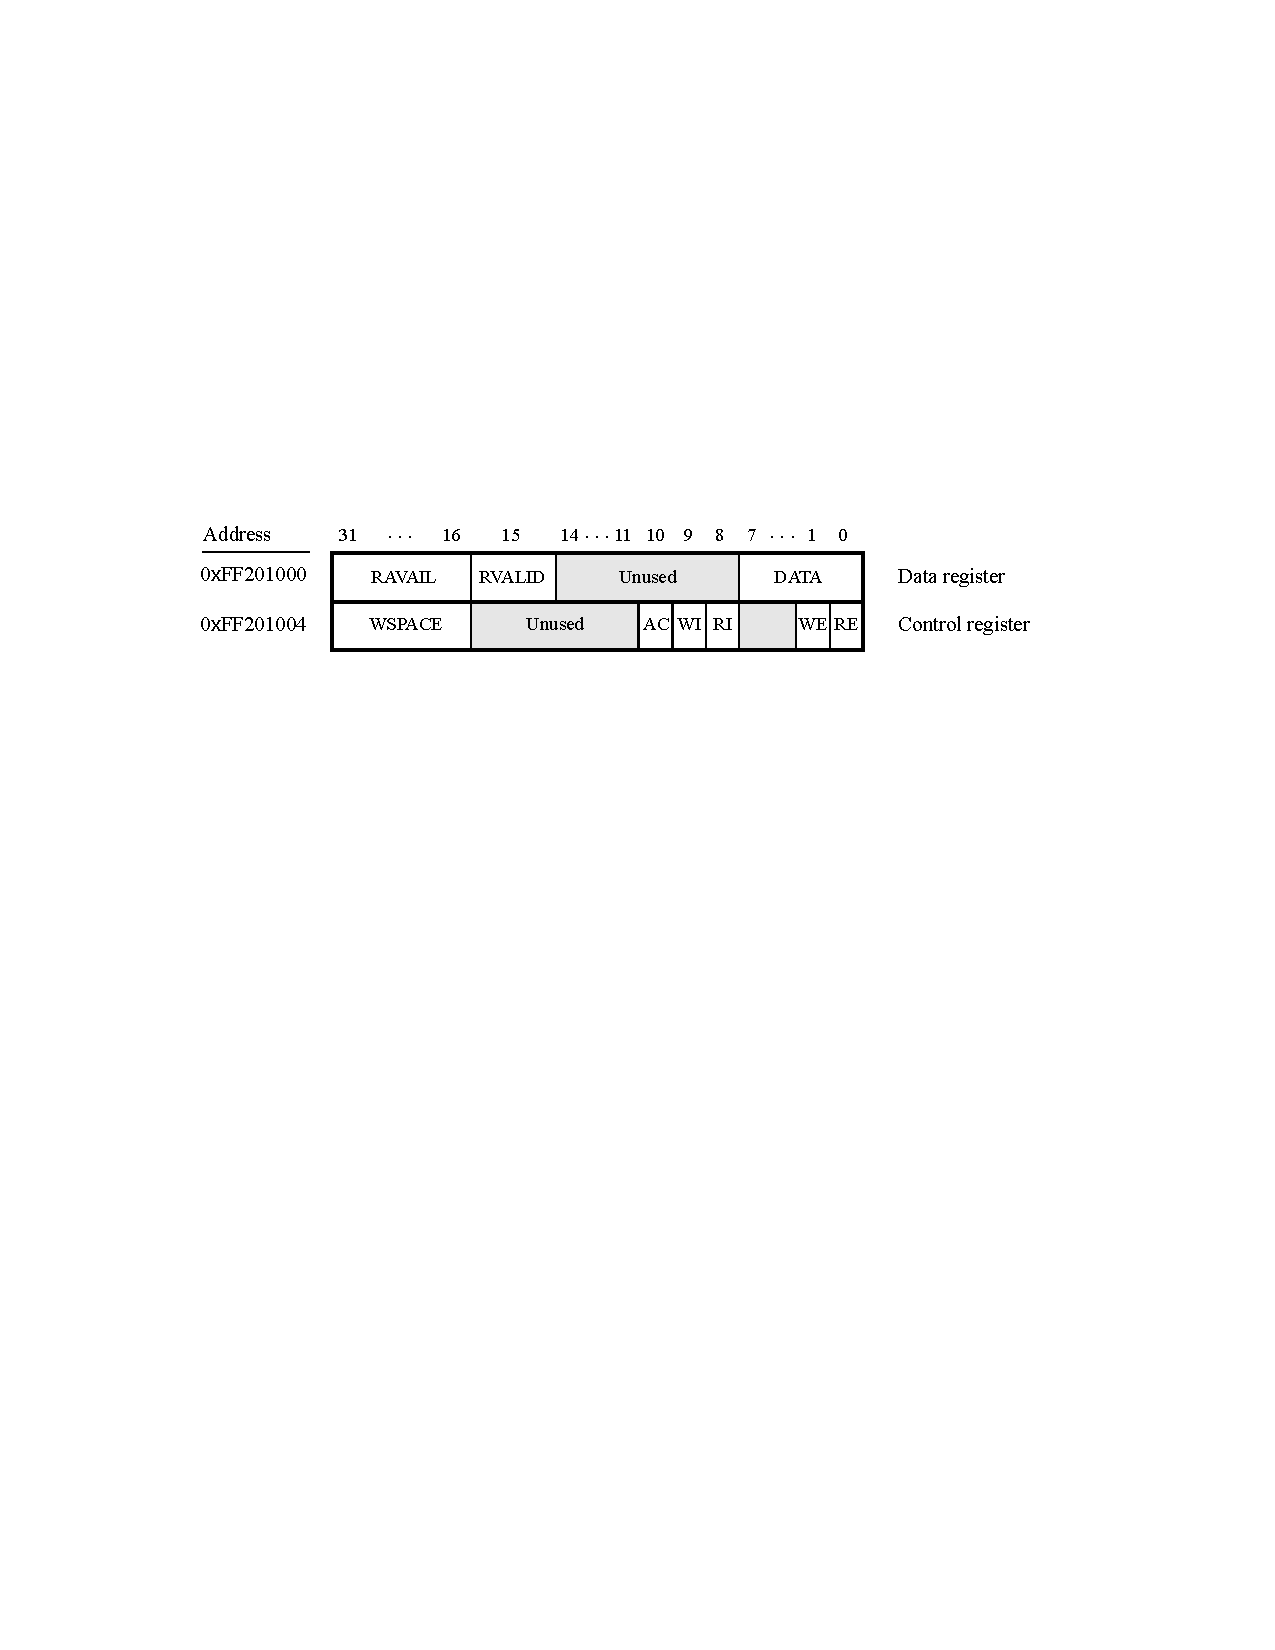
\includegraphics{../../../common/figs/FPGA_JTAG_UART.pdf}
   \end{center}
   \caption{JTAG UART registers.}
	\label{fig:jtag_port}
\end{figure}

When character data from the host computer is received by the JTAG UART 
it is stored in a 64-character FIFO.  The number of characters currently stored in this FIFO is
indicated in the field {\it RAVAIL}, which are
bits 31$-$16 of the {\it Data} register.  If the receive FIFO overflows, then
additional
data is lost. When data is present in the receive FIFO, then the value of {\it RAVAIL} will be 
greater than 0 and the value of bit 15, {\it RVALID}, will be 1. Reading the character at
the head of the FIFO, which is provided in bits $7-0$, decrements the value of {\it RAVAIL} 
by one and returns this decremented value as part of the read
operation. If no data is present in the receive FIFO, then {\it RVALID} will 
be set to 0 and the data in bits $7-0$ is undefined.

The JTAG UART also includes a 64-character FIFO that stores data 
waiting to be transmitted to the host computer. 
Character data is loaded into this FIFO by performing a write to bits 7$-$0
of the {\it Data} register in Figure \ref{fig:jtag_port}.  
Note that writing into this register has no effect 
on received data.  The amount of space, {\it WSPACE}, currently available in the transmit FIFO is 
provided in bits 31$-$16 of the {\it Control} register.  If
the transmit FIFO is full, then any characters written to the {\it Data} register will be lost.

Bit 10 in the {\it Control} register, called {\it AC}, has the value 1 if the JTAG UART has been
accessed by the host computer. This bit can be used to check if a working connection to
the host computer has been established. The {\it AC} bit can be cleared to 0 by writing a 1
into it.

The {\it Control} register bits {\it RE}, {\it WE}, {\it RI}, and {\it WI} are described 
in Section \ref{sec:exceptions}.

\subsubsection{Using the JTAG UART with Assembly Language Code and C Code}

Figures \ref{fig:jtag_uart_s} and \ref{fig:jtag_uart_C} give simple examples of 
assembly language and C code, respectively, that use the JTAG UART. Both versions of the
code perform the same function, which is to first send an ASCII string to the JTAG UART,
and then enter an endless loop. In the loop, the code reads character data that has 
been received by the JTAG UART, and echoes this data back to the UART for transmission. If the 
program is executed by using the \productNameMed{}, then any keyboard character that 
is typed into the {\it Terminal Window} of the Monitor Program will be 
echoed back, causing the character to appear in the {\it Terminal Window}.

The source code files shown in Figures \ref{fig:jtag_uart_s} and \ref{fig:jtag_uart_C}
are made available as part of the  
\productNameMed{}. The files can be found under the heading {\it sample programs}, 
and are identified by the name {\it JTAG UART}.

\begin{figure}[h!]
\lstset{style=defaultNiosStyle}
\begin{center}
\begin{minipage}[t]{12.5 cm}
\begin{tabbing}
/\=*****\=*********************************\=****************************************\=\kill
/********************************************************************************\\
\>* This program demonstrates the use of parallel ports in the DE1-SoC Computer:\\
\>* \>1. displays the SW switch values on the red LEDR\\
\>* \>2. displays a rotating pattern on the HEX displays\\
\>* \>3. if any KEY is pressed, the SW switches are used as the rotating pattern\\
\=\kill
\>********************************************************************************/\\
ZZZZZZZZ\={\bf movia}ZZZ\=r16, 0xFF200000ZZZZZZZZ\=/* RED\_LED base address */\kill
\>.{\bf text}	\>\>/* executable code follows */\\
\>.{\bf global} \>\_start\\
\_start:\\
\>/* initialize base addresses of parallel ports */\\
\>{\bf movia} \>r15, 0xFF200040 \>/* SW slider switch base address */\\
\>{\bf movia} \>r16, 0xFF200000 \>/* red LED base address */\\
\>{\bf movia} \>r17, 0xFF200050 \>/* pushbutton KEY base address */\\
\>{\bf movia} \>r20, 0xFF200020 \>/* HEX3\_HEX0 base address */\\
\>{\bf movia} \>r19, HEX\_bits\\
\>{\bf ldwio} \>r6, 0(r19) \>/* load pattern for HEX displays */\\
\rule{6.0in}{0in}~\\
DO\_DISPLAY:\\
\>{\bf ldwio} \>r4, 0(r15) \>/* load input from slider switches */\\
\>{\bf stwio} \>r4, 0(r16) \>/* write to red LEDs */\\
\>{\bf ldwio} \>r5, 0(r17) \>/* load input from pushbuttons */\\
\>{\bf beq} \>r5, r0, NO\_BUTTON\\
\>{\bf mov} \>r6, r4 \>/* copy SW switch values onto HEX displays */\\
WAIT:\\
\>{\bf ldwio} \>r5, 0(r17) \>/* load input from pushbuttons */\\
\>{\bf bne} \>r5, r0, WAIT \>/* wait for button release */\\
NO\_BUTTON:\\
\>{\bf stwio} \>r6, 0(r20) \>/* store to HEX3 ... HEX0 */\\
\>{\bf roli} \>r6, r6, 1 \>/* rotate the displayed pattern */\\
\>{\bf movia} \>r7, 500000 \>/* delay counter */\\
DELAY:	\\
\>{\bf subi} \>r7, r7, 1\\
\>{\bf bne} \>r7, r0, DELAY	\\
\>{\bf br} \>DO\_DISPLAY\\
~\\
\>.{\bf data}	\>\>/* data follows */\\
HEX\_bits:\\
\>.{\bf word} \>0x0000000F\\
\>.{\bf end}\\
\end{tabbing}
\end{minipage}
\end{center}
	\vspace{-0.33in}\caption{An example of assembly language code that uses the JTAG UART
	(Part {\it a}).}
   \label{fig:jtag_uart_s}
\end{figure}
\pagebreak
\clearpage
\newpage

\begin{center}
\begin{minipage}[t]{12.5 cm}
\begin{tabbing}
/\=*****\=***\=******************************\=****************************************\=\kill
/********************************************************************************\\
\>* Subroutine to send a character to the JTAG UART\\
\>* \>r5 \>= character to send\\
\>* \>r6 \>= JTAG UART base address\\
\=\kill
\>********************************************************************************/\\
ZZZZZZZZ\={\bf movia}ZZZ\=r16, 0xFF200000ZZZZZ\=/* RED\_LED base address */\kill
\>.{\bf global} \>PUT\_JTAG\\
PUT\_JTAG:\\
\>/* save any modified registers */\\
\>{\bf subi} \>sp, sp, 4 \>/* reserve space on the stack */\\
\>{\bf stw} \>r4, 0(sp) \>/* save register */\\
\\
\>{\bf ldwio} \>r4, 4(r6) \>/* read the JTAG UART Control register */\\
\>{\bf andhi} \>r4, r4, 0xffff \>/* check for write space */\\
\>{\bf beq} \>r4, r0, END\_PUT \>/* if no space, ignore the character */\\
\>{\bf stwio} \>r5, 0(r6) \>/* send the character */\\
\rule{6.0in}{0in}~\\
END\_PUT:\\
\>/* restore registers */\\
\>{\bf ldw} \>r4, 0(sp)\\
\>{\bf addi} \>sp, sp, 4\\
\\
\>{\bf ret}\\
\\
\>.{\bf data} \>\>/* data follows */\\
TEXT\_STRING:\\
\>.{\bf asciz} "$\backslash$nJTAG UART example code$\backslash$n$>$ "\\
\\
\>.{\bf end}\\
~\\
Figure \ref{fig:jtag_uart_s}. An example of assembly language code that uses the JTAG
UART (Part {\it b}).
\end{tabbing}
\end{minipage}
\end{center}
\pagebreak
\clearpage
\newpage
\begin{figure}[h!]
\begin{center}
\begin{minipage}[t]{12.5 cm}
\begin{tabbing}
ZZ\=ZZ\=ZZ\=HEX\_bits = HEX\_bits z 0xFFFFFFFF;ZZ\=// invert pattern for HEX displays\kill
/* function prototypes */\\
{\bf void} put\_jtag({\bf char});\\
{\bf char} get\_jtag({\bf void});\\
/\=*****\=*********************************\=****************************************\=\kill
/********************************************************************************\\
\>* This program demonstrates use of the JTAG UART port\\
\>* It performs the following: \\
\>* \>1. sends a text string to the JTAG UART\\
\>* \>2. reads and echos character data from/to the JTAG UART\\
\=\kill
\>********************************************************************************/\\
{\bf int} main({\bf void})\\
\{\\
ZZ\=ZZ\=ZZ\=HEX\_bits = HEX\_bits z 0xFFFFFFFF;ZZ\=// invert pattern for HEX displays\kill
\>{\bf char} text\_string[$\,$] = "$\backslash$nJTAG UART example code$\backslash$n$>$ $\backslash$0";\\
\>{\bf char} *str, c;\\
~\\
\>/* print a text string */\\
\>{\bf for} (str = text\_string; *str != 0; ++str)\\
\>\>put\_jtag (*str);
~\\
\>/* read and echo characters */\\
\>{\bf while} (1)\\
\>\{\\
\>\>c = get\_jtag ( );\\
\>\>{\bf if} (c != '$\backslash$0')\\
\>\>\>put\_jtag (c);\\
\>\}\\
\}
\rule{6.0in}{0in}~\\\\
/\=*****\=*********************************\=****************************************\=\kill
/********************************************************************************\\
\>* Subroutine to send a character to the JTAG UART\\
\=\kill
\>********************************************************************************/\\
ZZ\=ZZZ\=ZZZ\=HEX\_bits = HEX\_bits z ;ZZ\=// invert pattern for HEX displays\kill
{\bf void} put\_jtag( {\bf char} c )\\
\{\\
\>{\bf volatile int} * JTAG\_UART\_ptr 	= (int *) 0xFF201000;  // JTAG UART address\\
\>{\bf int} control;\\
\>control = *(JTAG\_UART\_ptr + 1);	\>\>\>// read the JTAG\_UART control register\\
\>{\bf if} (control \& 0xFFFF0000) \>\>\>// if space, echo character, else ignore \\
\>\>*(JTAG\_UART\_ptr) = c;\\
\}\\
\end{tabbing}
\end{minipage}
\end{center}
	\vspace{-0.33in}\caption{An example of C code that uses the JTAG UART (Part {\it a}).}
   \label{fig:jtag_uart_C}
\end{figure}
\pagebreak
\clearpage
\newpage
\begin{figure}[h!]
\begin{center}
\begin{minipage}[t]{12.5 cm}
\begin{tabbing}
/\=*****\=*********************************\=****************************************\=\kill
/********************************************************************************\\
\>* Subroutine to read a character from the JTAG UART\\
\>* Returns $\backslash$0 if no character, otherwise returns the character\\
\=\kill
\>********************************************************************************/\\
ZZ\=ZZZ\=ZZZ\=HEX\_bits = HEX\_bits z ;ZZ\=// invert pattern for HEX displays\kill
{\bf char} get\_jtag( {\bf void} )\\
\{\\
\>{\bf volatile int} * JTAG\_UART\_ptr	= ({\bf int} *) 0xFF201000;	// JTAG UART address\\
\>{\bf int} data;\\
\>data = *(JTAG\_UART\_ptr); \>\>\>// read the JTAG\_UART data register\\
\>{\bf if} (data \& 0x00008000) \>\>\>// check RVALID to see if there is new data\\
\>\>{\bf return} (({\bf char}) data \& 0xFF);\\
\>{\bf else}\\
\>\>{\bf return} ('$\backslash$0');\\
\}
~\\
\centerline{Figure \ref{fig:jtag_uart_C}. An example of C code that uses the JTAG UART (Part {\it b}).}
\end{tabbing}
\end{minipage}
\end{center}
\end{figure}
